\documentclass{beamer}

\usepackage[T2A]{fontenc}
\usepackage[utf8]{inputenc}
\usepackage[english,russian]{babel}
\input{settings.tex}
\usepackage{multicol}


\title{Линейные неравенства, Политопы}
\subtitle{Вычислительный интеллект, лекция 5}
\author{Сергей Савин}
\centering
\date{\mydate}

\begin{document}
\maketitle

%\begin{frame}{Содержание}
%	
%	\begin{itemize}
%		\item Выпуклые многогранники (polytopes)
%		\item Полупространства
%		\item H-представление
%		\item V-представление
%		\item G-представление (Зонотопы)
%		\item Линейная аппроксимация выпуклых областей
%	\end{itemize}
%	
%\end{frame}



\begin{frame}{Выпуклые многогранники, 1}
	\begin{flushleft}
		
		Прежде чем дать определение выпуклого многогранника, рассмотрим примеры:
		
		\include{fig1}
		
	\end{flushleft}
\end{frame}


\begin{frame}{Выпуклые многогранники, 2}
	\begin{flushleft}
		
		Можно представлять себе многогранники как геометрические фигуры (непрерывные множества точек) с плоскими (линейными) рёбрами, гранями и их многомерными аналогами.
		
		\bigskip
		
		\begin{definition}
			Выпуклый многогранник (convex polytope) — это ограниченное выпуклое множество, которое может быть представлено как пересечение конечного числа полупространств.
		\end{definition}
		
		\bigskip
		
		Если множество неограничено, мы называем его \emph{полиэдром} (polyhedron).
		
	\end{flushleft}
\end{frame}


\begin{frame}{Полупространства, Определение}
	\begin{flushleft}
		
		Мы можем определить полупространство как множество всех точек $\mathbf{x}$, таких что $\mathbf{a}^\top \mathbf{x} \leq b$. На следующем изображении закрашенное пространство \textbf{не} входит в полупространство.
		
		\include{fig2}
		
	\end{flushleft}
\end{frame}



\begin{frame}{Полупространство, проходящее через 0}
	\begin{flushleft}
		
		Рассмотрим полупространство, проходящее через начало координат и заданное своим вектором нормали $\mathbf{n}$:
		
		\include{fig3}
		
		Это полупространство можно определить как «все векторы $\mathbf{x}$, такие что $\mathbf{n} \cdot \mathbf{x} \leq 0$», что эквивалентно использованию $\mathbf{n}$ вместо $\mathbf{a}$ в исходном определении, при этом полагая $b = 0$.
		
	\end{flushleft}
\end{frame}




\begin{frame}{Полупространство, общий случай}
	\begin{flushleft}
		
		В общем случае существует некоторое расстояние между границей полупространства и началом координат, обозначим его $d$.
		
		\include{fig4}
		%
		Здесь полупространство можно определить как «все векторы $\mathbf{x}$, такие что $\mathbf{x}^\top \frac{\mathbf{n}}{|| \mathbf{n} ||}  \leq d$». Это эквивалентно тому, чтобы взять $\mathbf{a} = \mathbf{n}$ и $b = d ||\mathbf{n}||$.
		
	\end{flushleft}
\end{frame}


\begin{frame}{Комбинация полупространств}
	\begin{flushleft}
		
		Мы можем определить выпуклое множество как \emph{пересечение} полупространств $\mathbf{a}_i^\top \mathbf{x} \leq b_i$:
		
		\include{fig5}
		
		Результирующая область описывается как $\begin{bmatrix} \mathbf{a}_1^\top \\ ... \\ \mathbf{a}_k^\top \end{bmatrix} \mathbf{x} \leq \begin{bmatrix} b_1 \\ ... \\ b_k \end{bmatrix}$
		
		
	\end{flushleft}
\end{frame}


\begin{frame}{H-представление многогранника}
	%\framesubtitle{}
	\begin{flushleft}
		
		Последний результат позволяет нам записать любой выпуклый многогранник в виде матричного неравенства:
		
		\begin{equation}
			\label{eq:ineq} 
			\mathbf{A} \mathbf{x} \leq  \mathbf{b} 
		\end{equation}
		
		И наоборот, любое матричное неравенство \eqref{eq:ineq} представляет собой либо пустое множество, либо выпуклый многогранник (ограниченный), либо выпуклый полиэдр (неограниченный).
		
		\bigskip
		
		\begin{definition}
			$\mathbf{A} \mathbf{x} \leq  \mathbf{b}$ называется \emph{H-представлением} (half-space representation) полиэдра.
		\end{definition}
		
	\end{flushleft}
\end{frame}



\begin{frame}{H-представление в задачах выпуклой оптимизации}
	\begin{flushleft}
		
		Мы можем использовать H-многогранник (полиэдр) в качестве ограничений в задачах выпуклой оптимизации. Например, следующая задача квадратичного программирования (QP) включает такое ограничение:
		
		\begin{equation}
			\begin{aligned}
				& \underset{\mathbf{x}}{\text{minimize}}
				& & \mathbf{x}^\top \mathbf{H} \mathbf{x} + \mathbf{f}^\top\mathbf{x}, \\
				& \text{subject to}
				& & \mathbf{A}\mathbf{x} \leq \mathbf{b}.
			\end{aligned}
		\end{equation}
		
	\end{flushleft}
\end{frame}



\begin{frame}{Пример}
	\begin{flushleft}
		{\small 
		Найдите положение робота $\bo{r} = [x, \ y]\T$ в комнате длиной $l$ и шириной $w$, ближайшее к желаемой точке $\bo{r}_d= [x_d, \ y_d]\T$; система координат совмещена с осями комнаты, центр комнаты находится в точке (0, 0).
		
		\bigskip
		
		\hspace{-0.2in}
		\textbf{Решение}. Геометрия комнаты накладывает 4 ограничения на $\bo{r}$:
		
		\begin{multicols}{2}
			\begin{enumerate}
				\item $\begin{bmatrix} 1 & 0 \end{bmatrix} \bo{r} \leq 0.5 l$
				\item $\begin{bmatrix} -1 & 0 \end{bmatrix}  \bo{r} \leq 0.5 l$
				\item $\begin{bmatrix} 0 & 1 \end{bmatrix}  \bo{r} \leq 0.5 w$
				\item $\begin{bmatrix} 0 & -1 \end{bmatrix}  \bo{r} \leq 0.5 w$
			\end{enumerate}
		\end{multicols}
		
		Решение принимает форму задачи квадратичного программирования (QP):
		
		\begin{equation}
			\begin{aligned}
				& \underset{x, y}{\text{minimize}}
				& & (x-x_d)^2 + (y-y_d)^2, \\
				& \text{subject to}
				& & \begin{bmatrix} 1 & 0 \\ -1 & 0 \\ 0 & 1 \\ 0 & -1 \end{bmatrix}
				\begin{bmatrix} x \\ y \end{bmatrix}
				\leq
				\begin{bmatrix} 0.5 l \\ 0.5 l \\ 0.5 w \\ 0.5 w \end{bmatrix}
			\end{aligned}
		\end{equation}}
		
	\end{flushleft}
\end{frame}



\begin{frame}{V-представление}
	\begin{flushleft}
		
		Выпуклые многогранники имеют альтернативные представления, такие как \emph{V-представление}. Оно заключается в представлении многогранника в виде набора его вершин.
		
		\begin{example}
			$V = \begin{bmatrix} -1 & -1 & 1 & 1 \\ -1 & 1 & 1 & -1 \end{bmatrix}$ является V-представлением квадрата.
		\end{example}
		
		\begin{example}
			$\begin{bmatrix} 1 & 0 \\ 0 & 1 \\ -1 & 0 \\ 0 & -1 \end{bmatrix}
			\begin{bmatrix} x_1 \\ x_2 \end{bmatrix} \leq
			\begin{bmatrix} 1 \\ 1 \\ 1 \\ 1 \end{bmatrix}$
			является H-представлением того же квадрата.
		\end{example}
		
	\end{flushleft}
\end{frame}


\begin{frame}{Выпуклая оболочка}
	\begin{flushleft}
		
		Для заданных точек $\bo{x}_1$, $\bo{x}_2$, ..., $\bo{x}_N$ их выпуклая оболочка задаётся формулой:
		
		\begin{equation}
			\mathcal{P} = \left \{  \bo{x} = \sum_{i=1}^{N} \alpha_i\bo{x}_i: \   \sum_{i=1}^{N} \alpha_i = 1, \  \alpha_i \geq 0 \right \}
		\end{equation}
		
		
		\bigskip
		
		Обратите внимание, что ограничения $\sum_{i=1}^{N} \alpha_i = 1$ и $\alpha_i \geq 0$ автоматически ограничивают $\alpha_i$ интервалом $[0, \ 1]$.
		
		\bigskip
		
		См. Приложение для иллюстрации этой формулы.
		
	\end{flushleft}
\end{frame}



\begin{frame}{V-представление в задачах выпуклой оптимизации}
	\begin{flushleft}
		
		Мы можем использовать V-многогранник в качестве ограничений в задачах выпуклой оптимизации. Например, следующая задача квадратичного программирования (QP) включает такое ограничение:
		
		\begin{equation}
			\begin{aligned}
				& \underset{\mathbf{x}}{\text{minimize}}
				& & \mathbf{x}^\top \mathbf{H} \mathbf{x} + \mathbf{f}^\top\mathbf{x}, \\
				& \text{subject to}
				& & \begin{cases}
					\mathbf{x} = \sum\limits_{i=1}^{n} \alpha_i  \mathbf{v}_i, \\
					\sum\limits_{i=1}^{n} \alpha_i = 1, \\
					\alpha_i \geq 0.
				\end{cases}
			\end{aligned}
		\end{equation}
		
		Заметим, что это ограничение приравнивает $\mathbf{x}$ к выпуклой комбинации вершин V-многогранника.
		
	\end{flushleft}
\end{frame}





\begin{frame}{Пример}
	\begin{flushleft}
		
		Найдите положение робота $\bo{r} = [x, \ y]\T$, ближайшее к желаемой точке $\bo{r}_d= [x_d, \ y_d]\T$, на огороженной территории. Забор соединяет точку $(-10, 0)$ с $(0, 10)$ с $(7, 7)$ с $(0, -10)$.
		
		\bigskip
		
		\textbf{Решение}:
		
		\begin{equation}
			\begin{aligned}
				& \underset{x, y}{\text{minimize}}
				& & (x-x_d)^2 + (y-y_d)^2, \\
				& \text{subject to}
				& & 
				\begin{cases}
					\begin{bmatrix} x \\y \end{bmatrix}
					=
					\alpha_1
					\begin{bmatrix} -10 \\0 \end{bmatrix}
					+
					\alpha_2
					\begin{bmatrix} 0 \\10 \end{bmatrix}
					+
					\alpha_3
					\begin{bmatrix} 7 \\7 \end{bmatrix}
					+
					\alpha_4
					\begin{bmatrix} 0 \\ -10 \end{bmatrix}
					\\
					\alpha_1 + \alpha_2 + \alpha_3 + \alpha_4 = 1
					\\
					\alpha_1 \geq 0 \\  \alpha_2 \geq 0 \\  \alpha_3 \geq 0 \\  \alpha_4 \geq 0
				\end{cases}
			\end{aligned}
		\end{equation}
		
	\end{flushleft}
\end{frame}



\begin{frame}{H- и V-представления}
	\begin{flushleft}
		
		Преобразование между H- и V-представлениями в общем случае является вычислительно сложной задачей.
		
		\bigskip
		
		\begin{itemize}
			\item H $\rightarrow$ V: перечисление вершин (нахождение всех крайних точек)
			\item V $\rightarrow$ H: перечисление граней (нахождение всех определяющих неравенств)
		\end{itemize}
		
		
	\end{flushleft}
\end{frame}




\begin{frame}{Зонотопы: G-представление}
	\begin{flushleft}
		
		Зонотоп $\mathcal{Z}$ — это центрально-симметричный выпуклый многогранник, определяемый своим \emph{центром} $\bo{c}$ и \emph{матрицей генераторов} $\bo{G}$:
		
		\begin{equation}
			\mathcal{Z} = \{ \bo{x}: \ \bo{x}=\bo{G}\beta+\bo{c}, \ ||\beta||_\infty \leq 1  \}
		\end{equation}
		
		Множество $\{ \beta: \ ||\beta||_\infty \leq 1  \}$ является гиперкубом, а зонотоп $\mathcal{Z}$ — это проекция (тень) этого гиперкуба на пространство меньшей размерности; проекция определяется матрицей $\bo{G}$.
		
		\begin{figure}
			\centering
			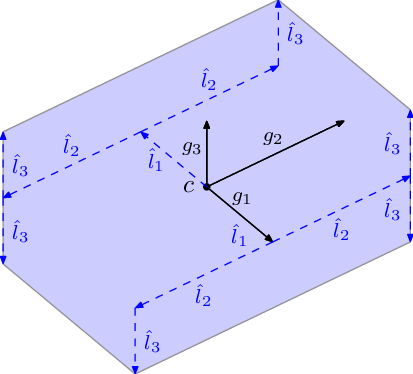
\includegraphics[width=0.4\linewidth]{zonotope_example}
			\caption{Зонотоп (\bref{https://www.researchgate.net/publication/322671928_Methods_for_order_reduction_of_zonotopes}{Источник}) }
			\label{fig:zonotopeexample}
		\end{figure}
		%https://www.researchgate.net/publication/322671928_Methods_for_order_reduction_of_zonotopes
		
		
	\end{flushleft}
\end{frame}




\begin{frame}{G-представление в задачах выпуклой оптимизации}
	\begin{flushleft}
		
		Мы можем использовать ограничение в виде зонотопа как часть задачи выпуклой оптимизации. Например, следующая задача квадратичного программирования (QP) включает такое ограничение:
		
		\begin{equation}
			\begin{aligned}
				& \underset{\mathbf{x}}{\text{minimize}}
				& & \mathbf{x}^\top \mathbf{H} \mathbf{x} + \mathbf{f}^\top\mathbf{x}, \\
				& \text{subject to}
				& & \begin{cases}
					\mathbf{x} = \bo{G}\beta+\bo{c}, \\
					-1 \leq \beta_i \leq 1.
				\end{cases}
			\end{aligned}
		\end{equation}
		
	\end{flushleft}
\end{frame}




\begin{frame}{\small{Линейная аппроксимация выпуклых областей}}
	\begin{flushleft}
		Некоторые выпуклые области могут быть легко аппроксимированы с помощью многогранников.
		
		\include{fig6}
		%
		Это позволяет нам представлять ограничения на принадлежность $\mathbf{x}$ к такой области в виде матричного неравенства
		
	\end{flushleft}
\end{frame}



\begin{frame}{Упражнение}
	\begin{flushleft}
		
		Запишите H-представление следующих многогранников:
		
		\begin{itemize}
			\item Равносторонний треугольник
			\item Квадрат
			\item Параллелепипед
			\item Трапеция
		\end{itemize}
		
	\end{flushleft}
\end{frame}

\myqrframe





\begin{frame}{Appendix A - convex hull, 1}
	\begin{flushleft}
		
		
		\begin{figure}[.45\textwidth]
			\centering
			\resizebox{.65\textwidth}{!}
			{\input{figure_convhull_0}}
		\end{figure}
		
		Let us illustrate the convex combination formula. 
		Let $\mathcal{P}$ be convex hull of points $\bo{x}_1$, $\bo{x}_2$ and $\bo{x}_3$:
		
		
		\begin{equation}
			\mathcal{P} = \left \{  \bo{x} = \sum_{i=1}^{3} \alpha_i\bo{x}_i: \   \sum_{i=1}^{3} \alpha_i = 1, \  \alpha_i \geq 0 \right \}
		\end{equation}
		
		Let $\bo{z}$ be a convex combination of $\bo{x}_1$ and $\bo{x}_3$: $\bo{z} = \beta_1 \bo{x}_1 + \beta_3 \bo{x}_3 $. Any point $\bo{p} \in \mathcal{P}$ can be defined as a convex combination of correctly chosen $\bo{z}$ and $\bo{x}_2$: $\bo{p} = \gamma_1 \bo{z} + \gamma_2 \bo{x}_2$.
		
	\end{flushleft}
\end{frame}



\begin{frame}{Appendix A - convex hull, 2}
	\begin{flushleft}
		
		
		
		\begin{figure}[.45\textwidth]
			\centering
			\resizebox{.45\textwidth}{!}
			{\input{figure_convhull_0}}
		\end{figure}
		
		We can express $\bo{p}$ as:
		%
		\begin{align}
			\bo{p} =  \gamma_1 \bo{z} + \gamma_2 \bo{x}_2 
			           = \gamma_1 (\beta_1 \bo{x}_1 + \beta_3 \bo{x}_3 )+ \gamma_2 \bo{x}_2
		\end{align}
		%
		We can define $\alpha_1 = \gamma_1 \beta_1$, $\alpha_2= \gamma_2$ and $\alpha_3 = \gamma_1 \beta_3$. Since $\gamma_i \geq 0$ and $\beta_i \geq 0$, we conclude that $\alpha_i \geq 0$.
		
		\bigskip
		
		We can show that:
		%
		\begin{align}
			\alpha_1 + \alpha_2+\alpha_3 =  \gamma_1(\beta_1 +\beta_3) + \gamma_2 = \gamma_1 + \gamma_2 = 1
		\end{align}
		
		
	\end{flushleft}
\end{frame}




\begin{frame}{Appendix A - convex hull, 3}
	\begin{flushleft}
		
		
					\begin{figure}
							\begin{subfigure}{.5\textwidth}
									\centering
									\resizebox{.95\textwidth}{!}
									{\input{figure_convhull_1}}
%									\label{fig:sfig1}
								\end{subfigure}%
							\begin{subfigure}{.5\textwidth}
									\centering
									\resizebox{.95\textwidth}{!}
									{\input{figure_convhull_2}}
%									\label{fig:sfig2}
								\end{subfigure}
%							\caption{plots of....}
%							\label{fig:fig}
						\end{figure}
		
		Previously we illustrated sufficiency of the formula's constraints. Now let us illustrate their necessity.
		
		\bigskip
		
		Dropping requirement $\alpha_i \geq 0$ and/or $\sum\limits_{i=1}^{3} \alpha_i = 1,$ leads to inclusion of points out the convex hull, as illustrated on the figures.
		
		
	\end{flushleft}
\end{frame}




\end{document}
